% !TEX root = ../final_report.tex
\appendix
\section*{Appendices}
\addcontentsline{toc}{section}{Appendices}
\renewcommand{\thesubsection}{\Alph{subsection}}

\subsection{Application Repository}
\label{appendix:code}
\rule{\textwidth}{0.4pt}

\subsubsection{Location}
The Git repository for this project is available here: \newline \url{https://github.com/StephenCoady/lifecycle-management-for-docker}.

\subsubsection{Contributing}
Since this project is open source anybody is welcome to contribute. To do so:
\begin{enumerate}
	\item Clone the repository
	\item Make a branch
	\item Make the changes you want
	\item Submit a pull request on your code
\end{enumerate}
Once the pull request has then been reviewed it will be merged into the main code base.
\subsubsection{Raising an issue}
If you find a bug, please raise an issue on Github and it will then be resolved as soon as possible. 

\subsubsection{Running the application}
If you wish to run the application please first clone the repository and then run `node index.js' from within the directory.

Alternatively, you can use Docker. To do this please follow the instructions found in the README.md file in the repository.
\clearpage

\subsection{Travis Repository} 
\label{appendix:travis}
\rule{\textwidth}{0.4pt}
\subsubsection{Location}
The repository can be found at:  \url{https://travis-ci.org/StephenCoady/lifecycle-management-for-docker}

\subsubsection{Build Statistics}
We can see some statistics for the builds of this project below in Figure \ref{fig:build-stats}.

\begin{figure}[!ht]
\centering
\includegraphics*[width=0.5\textwidth]{images/build-stats}
\caption{\em Project Build Statistics}
\label{fig:build-stats}
\end{figure}

We can also see the builds per day and average time take to complete a build below in Figures \ref{fig:builds-per-day} and \ref{fig:build-time}.

\begin{figure}[!ht]
\centering
\begin{minipage}{.5\textwidth}
  \centering
  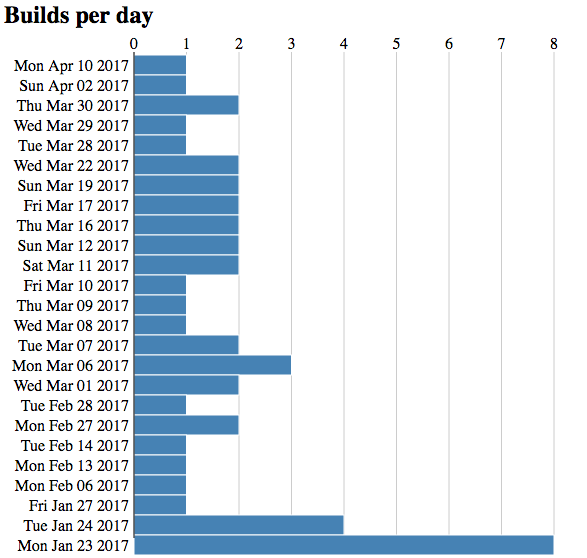
\includegraphics[width=\linewidth]{images/builds-per-day}
	\caption{\em Project Builds per Day}
	\label{fig:builds-per-day}
\end{minipage}%
\begin{minipage}{.5\textwidth}
  \centering
  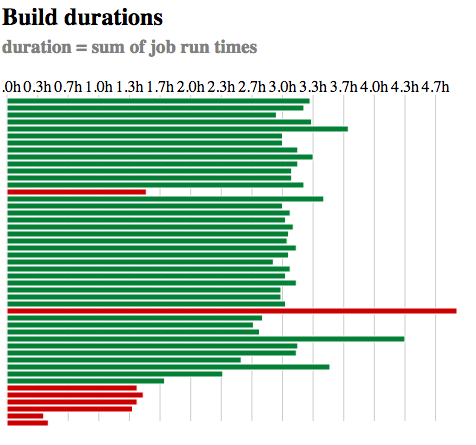
\includegraphics[width=\linewidth]{images/build-time}
	\caption{\em Project Average Build Time}
	\label{fig:build-time}
\end{minipage}
\end{figure}
\clearpage

\subsection{SonarQube Repository} 
\label{appendix:sonarqube}
\rule{\textwidth}{0.4pt}
\subsubsection{Location}
The SonarQube quality gate for this application can be found at:
\url{https://sonarqube.com/dashboard?id=lifecycle-management-for-docker}



\subsection{DockerHub Repository} 
\label{appendix:dockerhub}
https://hub.docker.com/r/scoady2/lifecycle-management-for-docker/

\subsection{Staging Server} 
\label{appendix:staging}
application: http://87.44.18.55:3000/ \newline
documentation: http://87.44.18.55:3000/docs

default username: admin \newline
default password: admin

\subsection{Dockerode} 
\label{appendix:dockerode_appendix}
https://github.com/apocas/dockerode

\subsection{Report Source Code} 
\label{appendix:reports}
https://github.com/StephenCoady/college-papers

\clearpage
\subsection{Formal System Models}
\label{appendix:models}

\begin{figure}[!ht]
\centering
\makebox[\textwidth]{\includegraphics*[width=0.9\paperwidth]{images/models/docker_class_diagram}}
\caption{\em Class Diagram}
\end{figure}

\begin{figure}[!ht]
\centering
\makebox[\textwidth]{\includegraphics*[width=0.9\paperwidth]{images/models/docker_system}}
\caption{\em Sequence Diagram}
\end{figure}

\begin{figure}[!ht]
\centering
\makebox[\textwidth]{\includegraphics*[width=0.8\paperwidth]{images/models/user_system}}
\caption{\em User System Sequence Diagram}
\end{figure}

\begin{figure}[!ht]
\centering
\makebox[\textwidth]{\includegraphics*[width=0.9\paperwidth]{images/models/use_case}}
\caption{\em Use Case Diagram}
\end{figure}

\clearpage

\subsection{Wireframes}
\label{appendix:wireframes}

\begin{figure}[!ht]
\centering
\includegraphics*[width=0.9\textwidth]{wireframes/dashboard}
\caption{\em Dashboard Mockup}
\end{figure}

\begin{figure}[!ht]
\centering
\includegraphics*[width=0.9\textwidth]{wireframes/container}
\caption{\em Container Mockup}
\end{figure}

\begin{figure}[!ht]
\centering
\includegraphics*[width=0.9\textwidth]{wireframes/images}
\caption{\em Images Mockup}
\end{figure}

\begin{figure}[!ht]
\centering
\includegraphics*[width=0.9\textwidth]{wireframes/image}
\caption{\em Image Mockup}
\end{figure}

\begin{figure}[!ht]
\centering
\includegraphics*[width=0.9\textwidth]{wireframes/networks}
\caption{\em Networks Mockup}
\end{figure}

\begin{figure}[!ht]
\centering
\includegraphics*[width=0.9\textwidth]{wireframes/network}
\caption{\em Network Mockup}
\end{figure}

\begin{figure}[!ht]
\centering
\includegraphics*[width=0.9\textwidth]{wireframes/docker}
\caption{\em Docker Mockup}
\end{figure}

\begin{figure}[!ht]
\centering
\includegraphics*[width=0.9\textwidth]{wireframes/host}
\caption{\em Host Mockup}
\end{figure}
